\section{Auswertung}
\label{sec:Auswertung}

Aus \autoref{tab:wertea} sind die Messwerte zu Aufgabenteil a) zu entnehmen.
\begin{table}[H]
    \centering
    \caption{Messwerte zur Wheatstone MessbrückeAufgabe a.}
    \label{tab:wertea}
    \begin{tabular}{c c}
        \toprule
        $U \:/\:$ V & $t \:/\:$ ms \\
        \midrule
        0,55 & 0,00 \\
        0,50 & 0,02 \\
        0,44 & 0,04 \\
        0,40 & 0,05 \\
        0,36 & 0,06 \\
        0,32 & 0,08 \\
        0,26 & 0,10 \\
        0,24 & 0,12 \\
        0,18 & 0,14 \\
        0,12 & 0,16 \\
        0,1 & 0,18 \\
        0,04 & 0,20 \\
        0,00 & 0,22 \\
        -0,04 & 0,24 \\
        -0,06 & 0,26 \\
        -0,10 & 0,28 \\
        -0,14 & 0,30 \\
        -0,16 & 0,32 \\
        -0,18 & 0,34 \\
        -0,22 & 0,36 \\
        -0,24 & 0,38 \\
        -0,28 & 0,40 \\
        -0,30 & 0,42 \\
        -0,32 & 0,44 \\
        -0,34 & 0,46 \\
        -0,38 & 0,48 \\
        -0,40 & 0,5 \\
        -0,42 & 0,52 \\
        -0,44 & 0,54 \\
        -0,46 & 0,56 \\
        -0,48 & 0,58 \\
        -0,50 & 0,6 \\
        \bottomrule
    \end{tabular}
\end{table}

Aus \autoref{tab:wertebc} sind die Messwerte zu Aufgabenteil b) und c) zu entnehmen.
\begin{table}[H]
    \centering
    \caption{Messwerte zu Aufgabe c) und b).}
    \label{tab:wertebc}
    \begin{tabular}{c c c c c}
        \toprule
        $f \:/\:\si{\kilo\hertz}$ & $A_1 \:/\: \si{\volt}$ & $A_1 \:/\: \si{\volt}$ & $a \:/\: \si{\milli\second}$ & $b \:/\: \si{\milli\second}$ \\
        \midrule
        0,2627 & 4,4 & 2,4000 & 0,0350 & 2,5500 \\
        3,085 & 4,2 & 0,1100 & 0,0300 & 0,1800 \\
        6 & 4,2 & 0,0600 & 0,0240 & 0,0680 \\
        9 & 4,2 & 0,0480 & 0,0180 & 0,070 \\
        12 & 4,2 & 0,0360 & 0,0120 & 0,0460 \\
        15 & 4,2 & 0,0260 & 0,0100 & 0,0380 \\
        18 & 4,2 & 0,0220 & 0,0100 & 0,0240 \\
        21 & 4,2 & 0,0180 & 0,0080 & 0,0260 \\
        24 & 4,2 & 0,0150 & 0,0070 & 0,0230 \\
        27 & 4,2 & 0,0130 & 0,0060 & 0,0210 \\
        30 & 4,2 & 0,0110 & 0,0050 & 0,0190 \\
        33 & 4,2 & 0,0100 & 0,0050 & 0,0165 \\
        36 & 4,2 & 0,0085 & 0,0050 & 0,0150 \\
        39 & 4,2 & 0,0075 & 0,0045 & 0,0114 \\
        42 & 4,2 & 0,0070 & 0,0040 & 0,0135 \\
        45 & 4,2 & 0,0060 & 0,0040 & 0,0120 \\
        48 & 4,2 & 0,0060 & 0,0035 & 0,0115 \\
        51 & 4,2 & 0,0050 & 0,0030 & 0,0110 \\
        54 & 4,2 & 0,0050 & 0,0030 & 0,0100 \\
        57 & 4,2 & 0,0045 & 0,0030 & 0,0100 \\
        60 & 4,2 & 0,0040 & 0,0025 & 0,0095 \\
        \bottomrule
    \end{tabular}
\end{table}


Aus \autoref{fig:entladekurve} ist eine Abbildung der Entladekurve auf einem Oszilloskop zu entnehmen.
\begin{figure}[H]
    \centering
    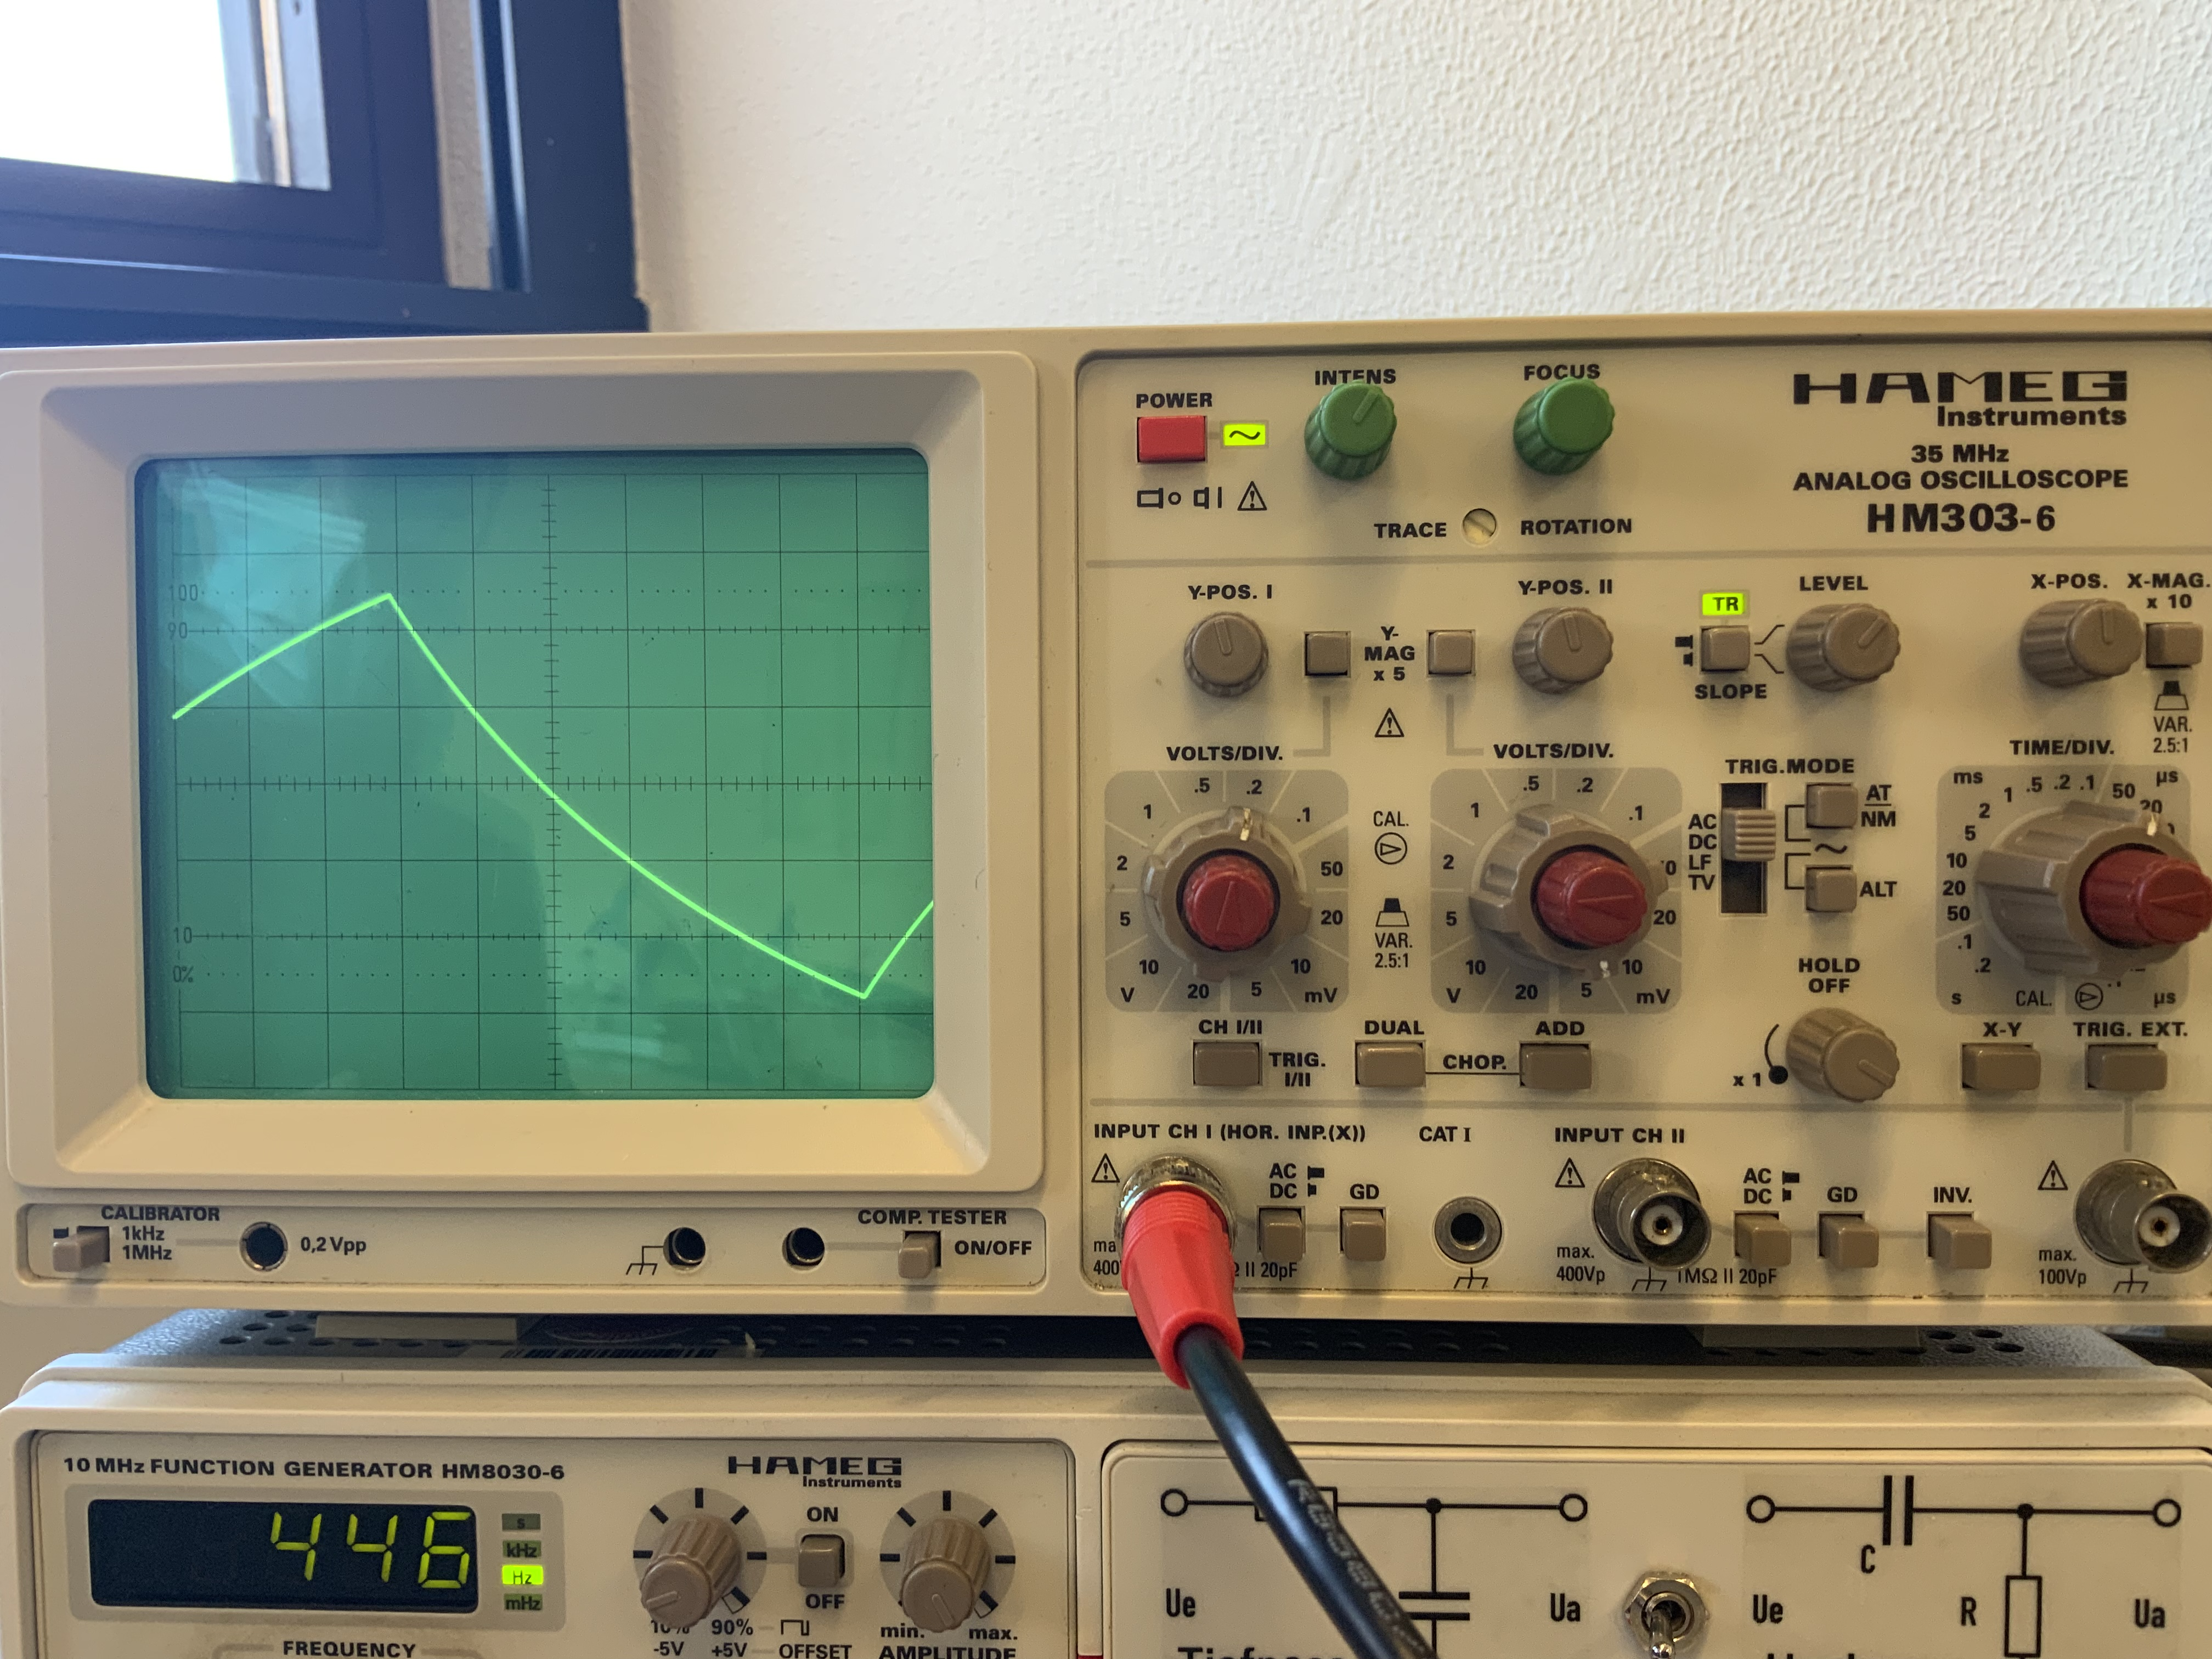
\includegraphics[width=0.75\textwidth]{Dateien/entladekurve.jpeg}
    \caption{Entladekurve.}
    \label{fig:entladekurve}
\end{figure}

Aus \autoref{fig:d.1}, \autoref{fig:d.2} und \autoref{fig:d.3} sind die Messwerte zu Aufgabenteil d) zu entnehmen.
\begin{figure}[H]
    \centering
    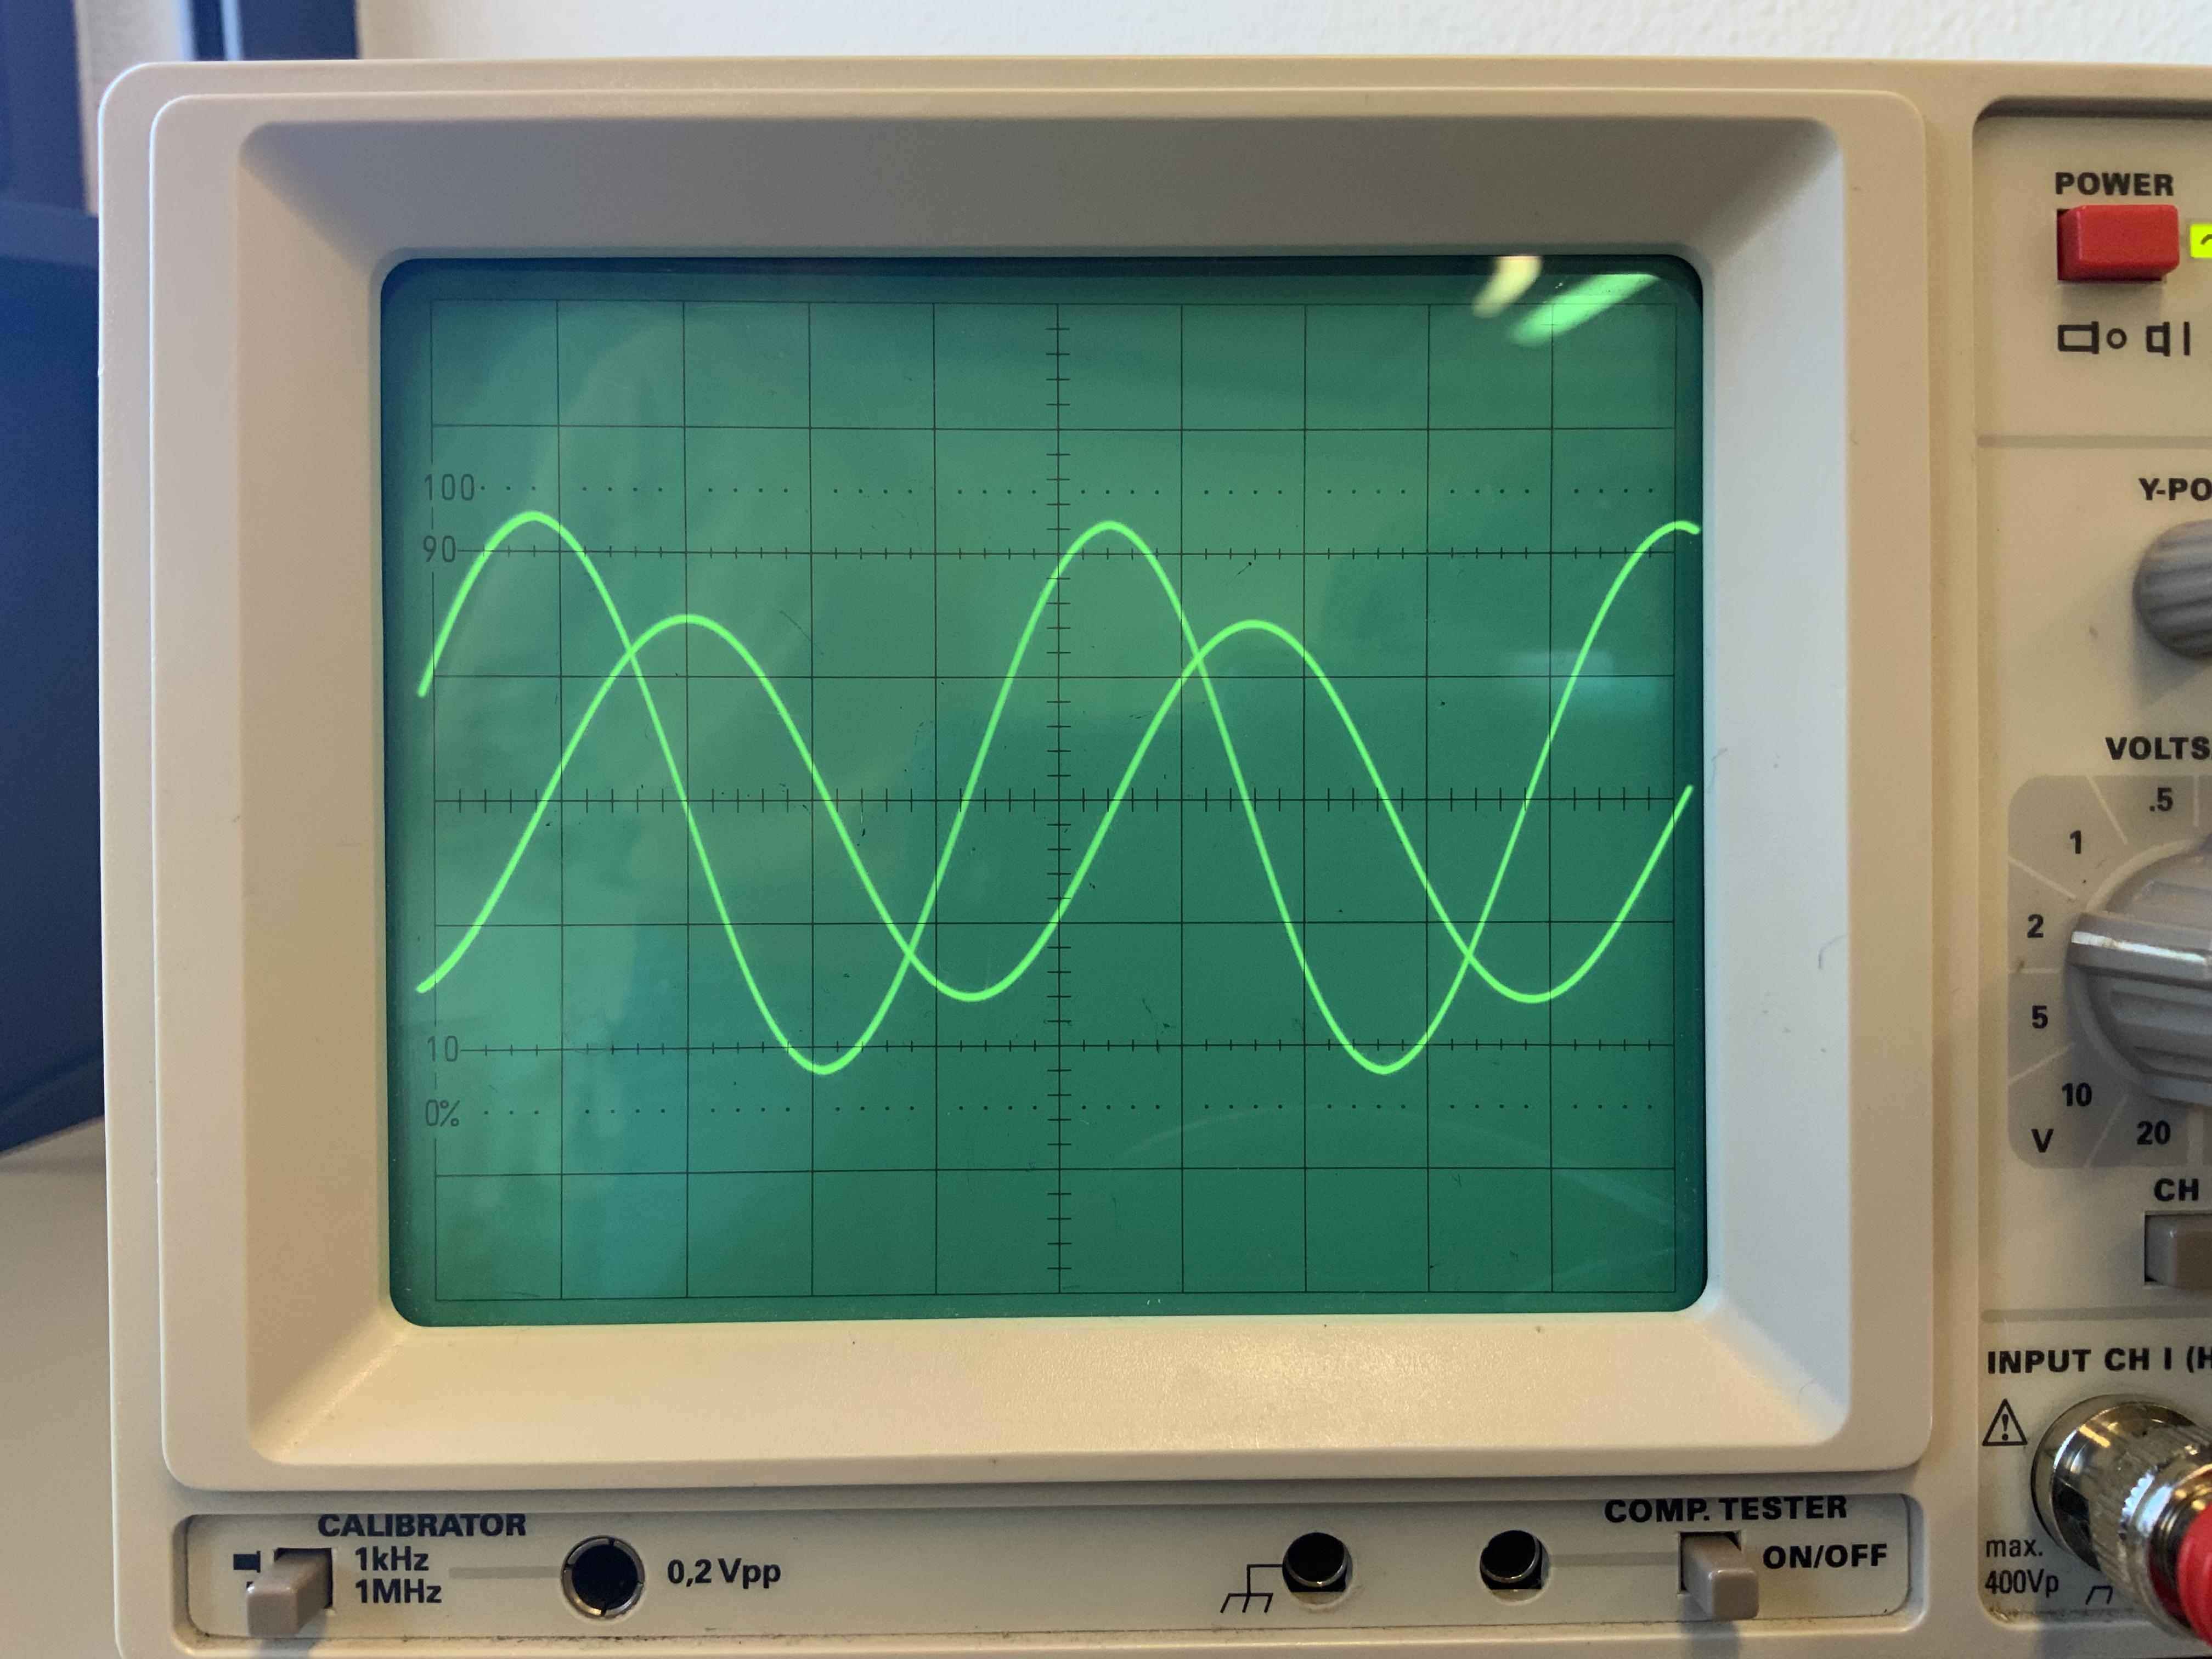
\includegraphics[width=0.75\textwidth]{Dateien/d.1.jpeg}
    \caption{Messdaten zu Aufgabenteil d).}
    \label{fig:d.1}
\end{figure}

\begin{figure}[H]
    \centering
    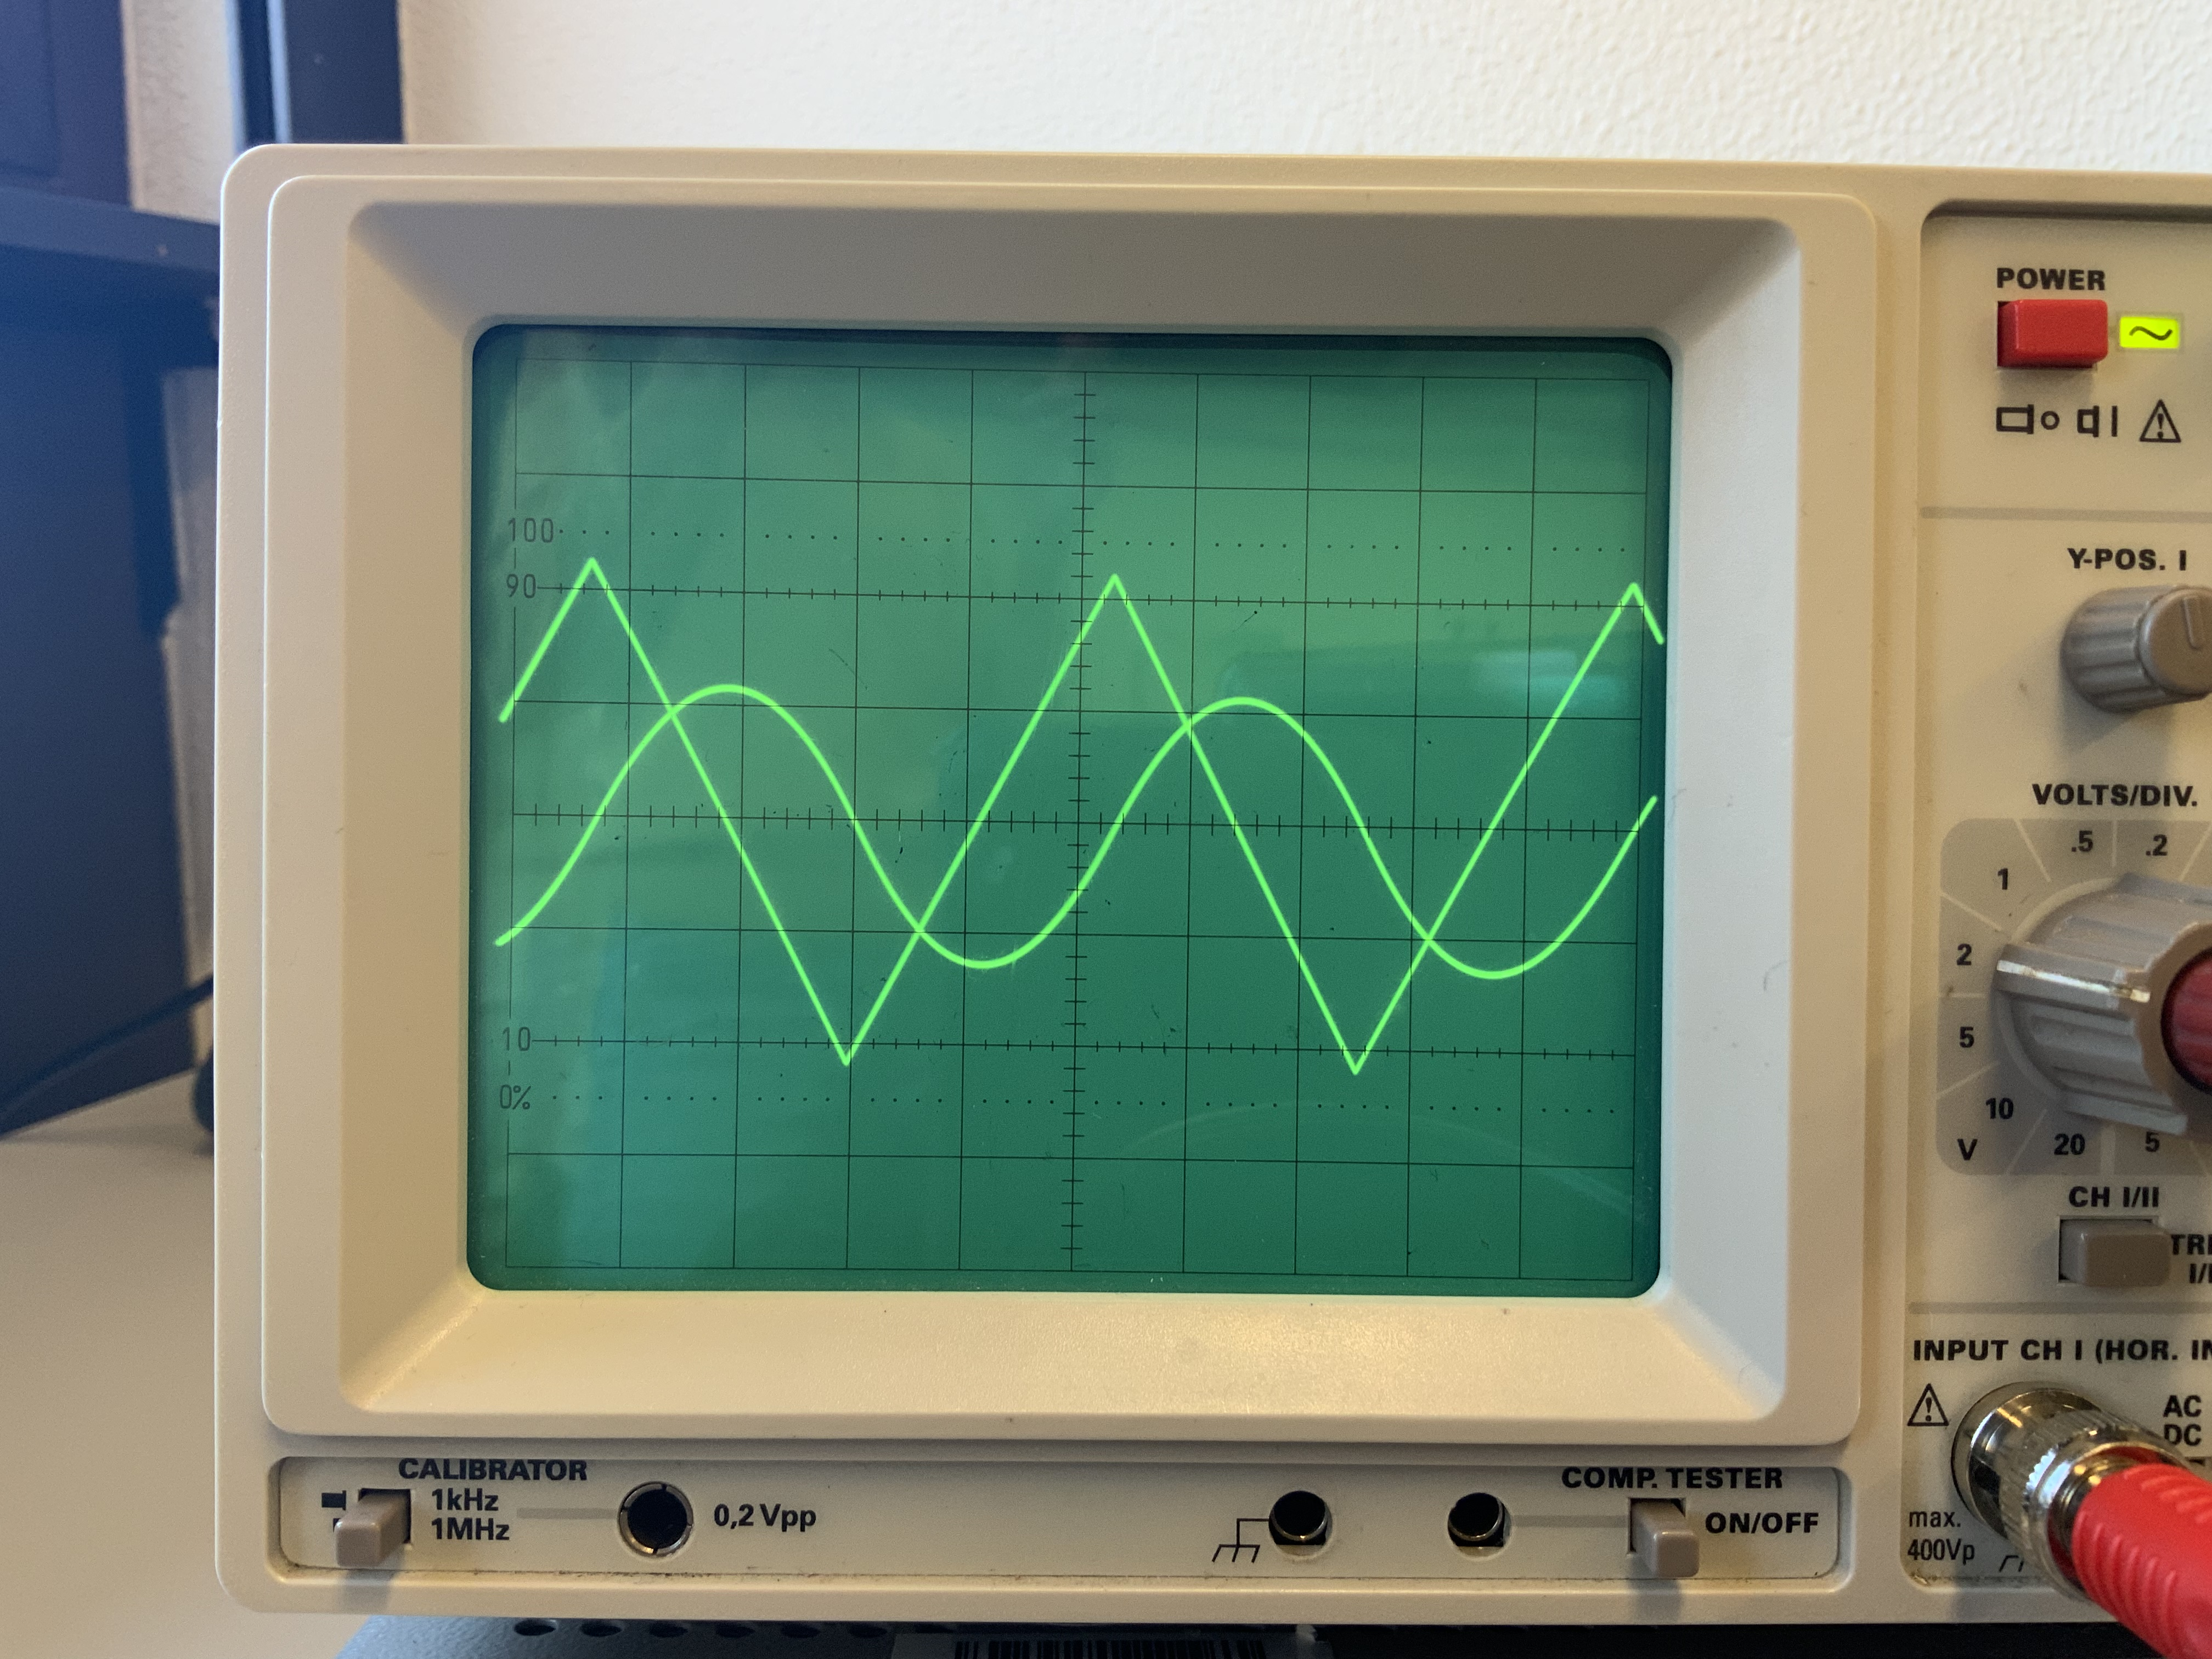
\includegraphics[width=0.75\textwidth]{Dateien/d.2.jpeg}
    \caption{Messdaten zu Aufgabenteil d).}
    \label{fig:d.2}
\end{figure}

\begin{figure}[H]
    \centering
    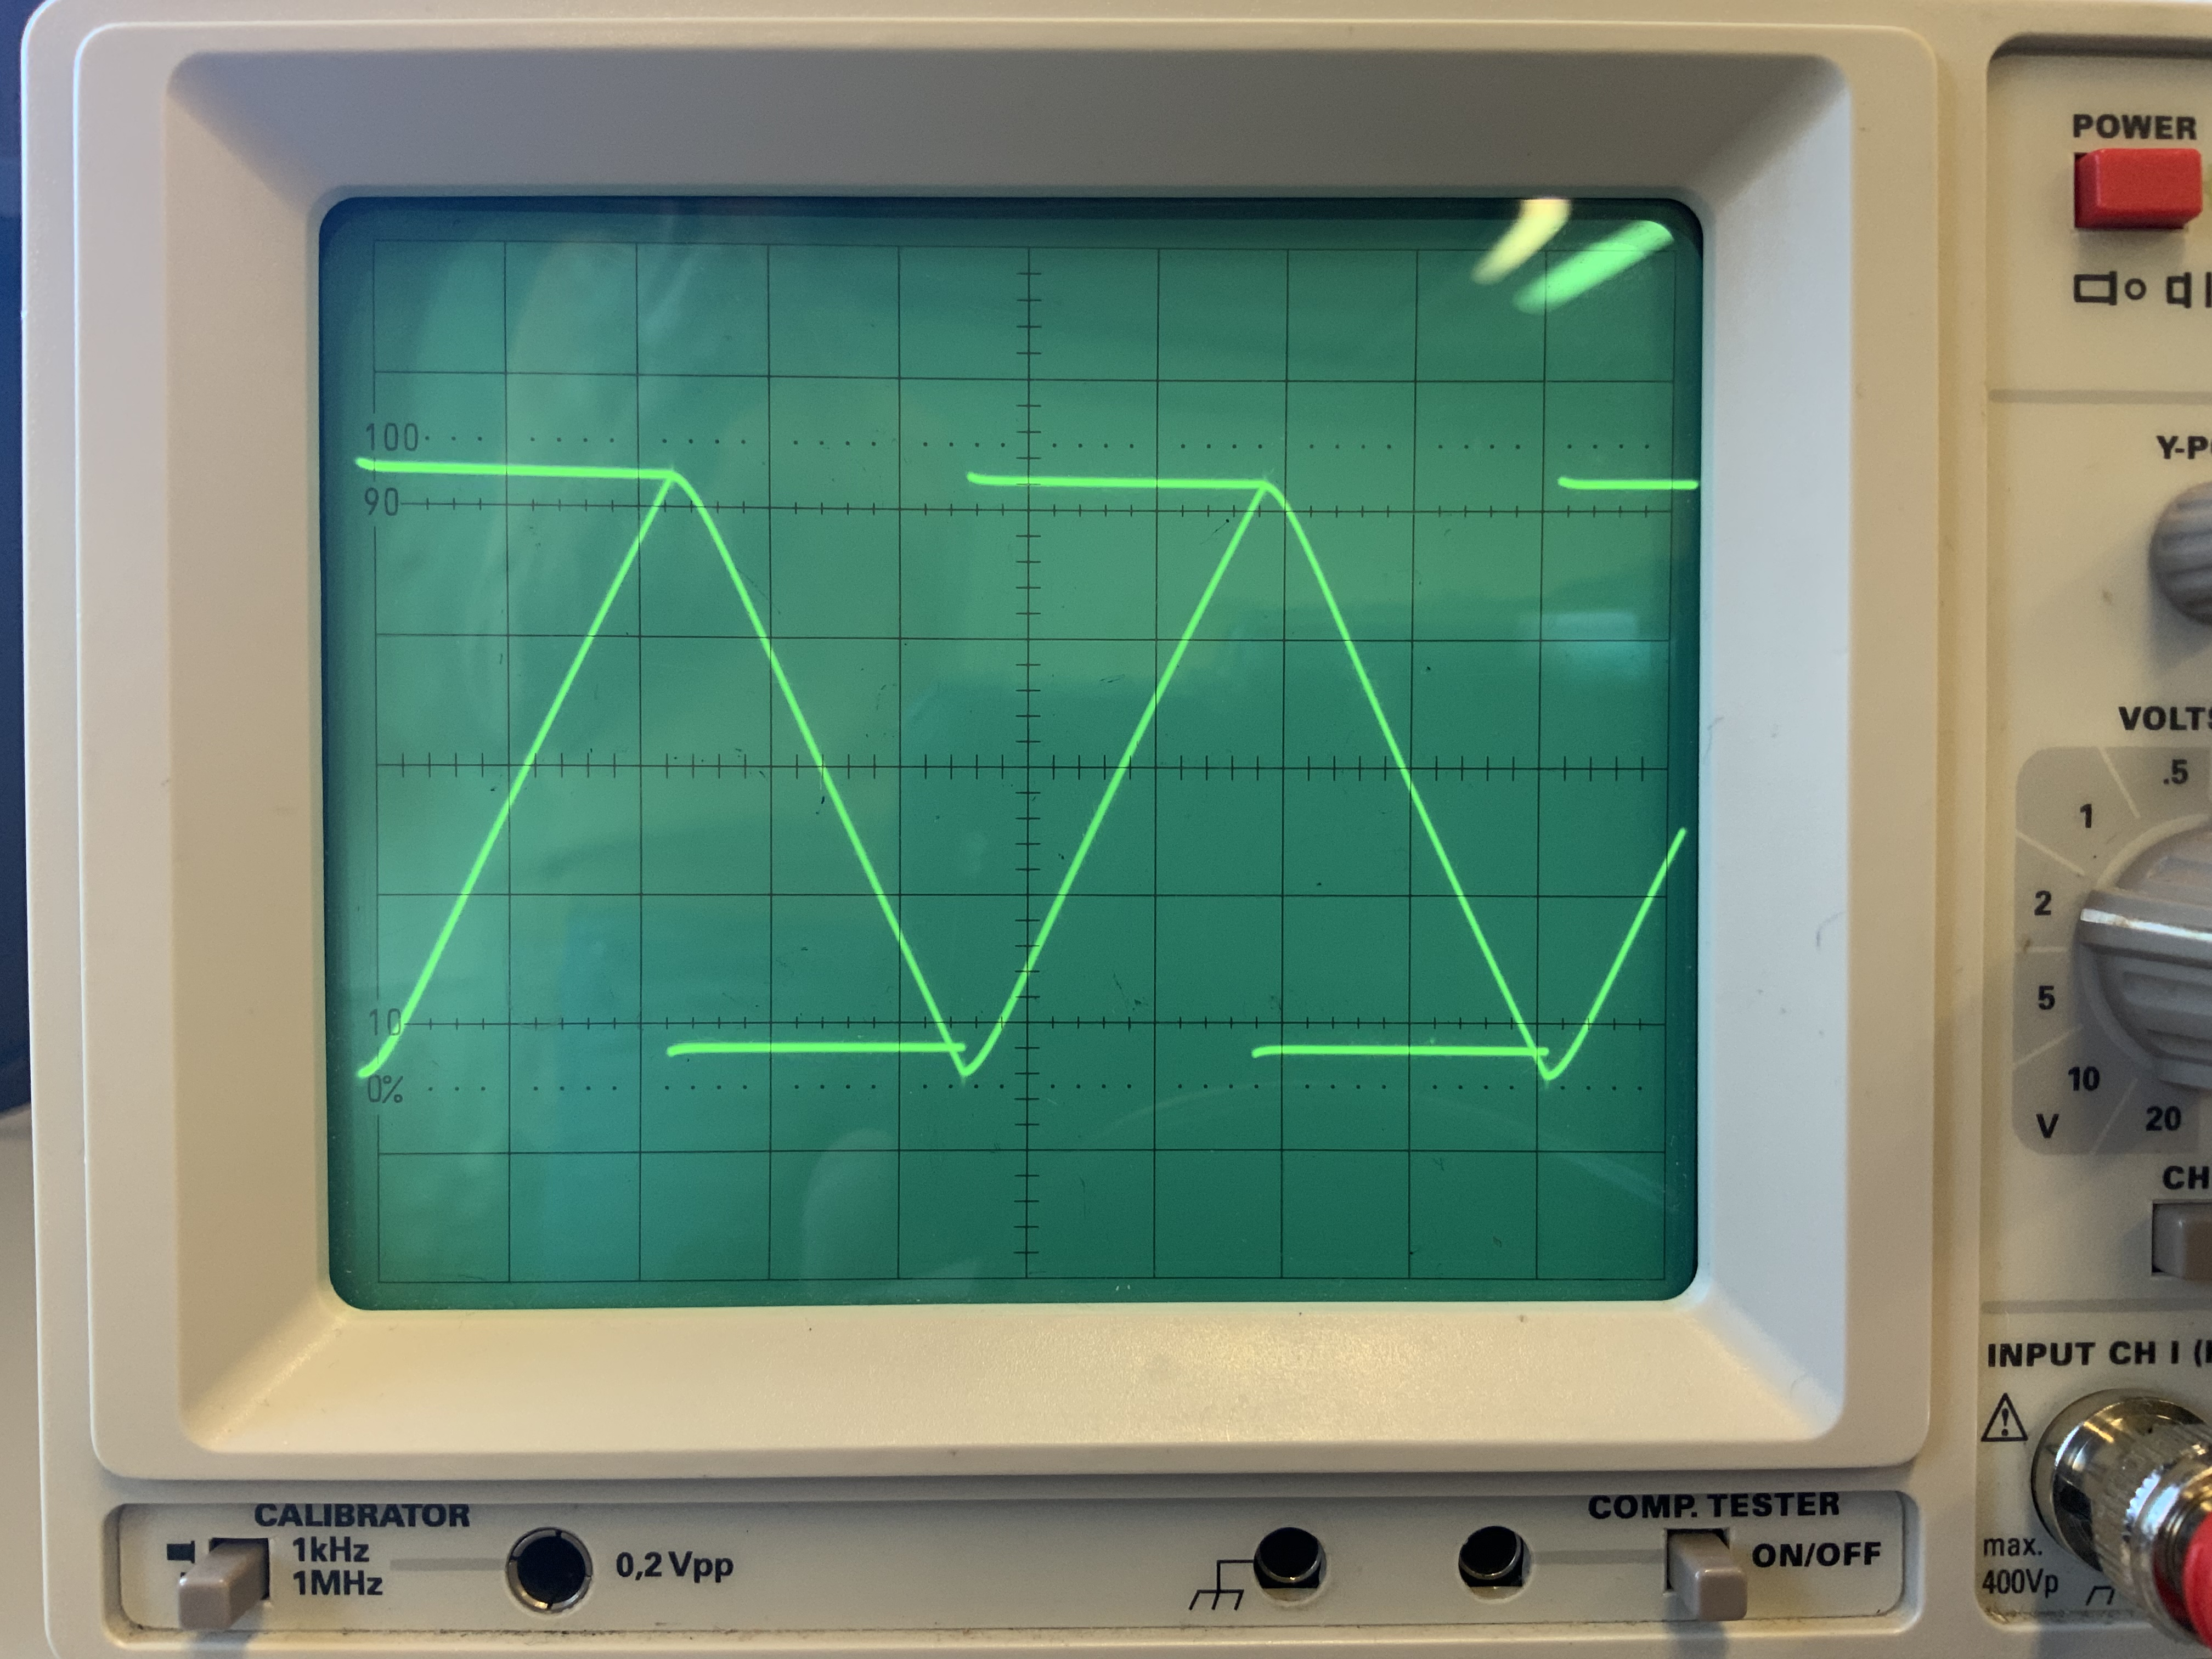
\includegraphics[width=0.75\textwidth]{Dateien/d.3.jpeg}
    \caption{Messdaten zu Aufgabenteil d).}
    \label{fig:d.3}
\end{figure}


%%%     Originale Messwerte
\begin{figure}[H]
    \centering
    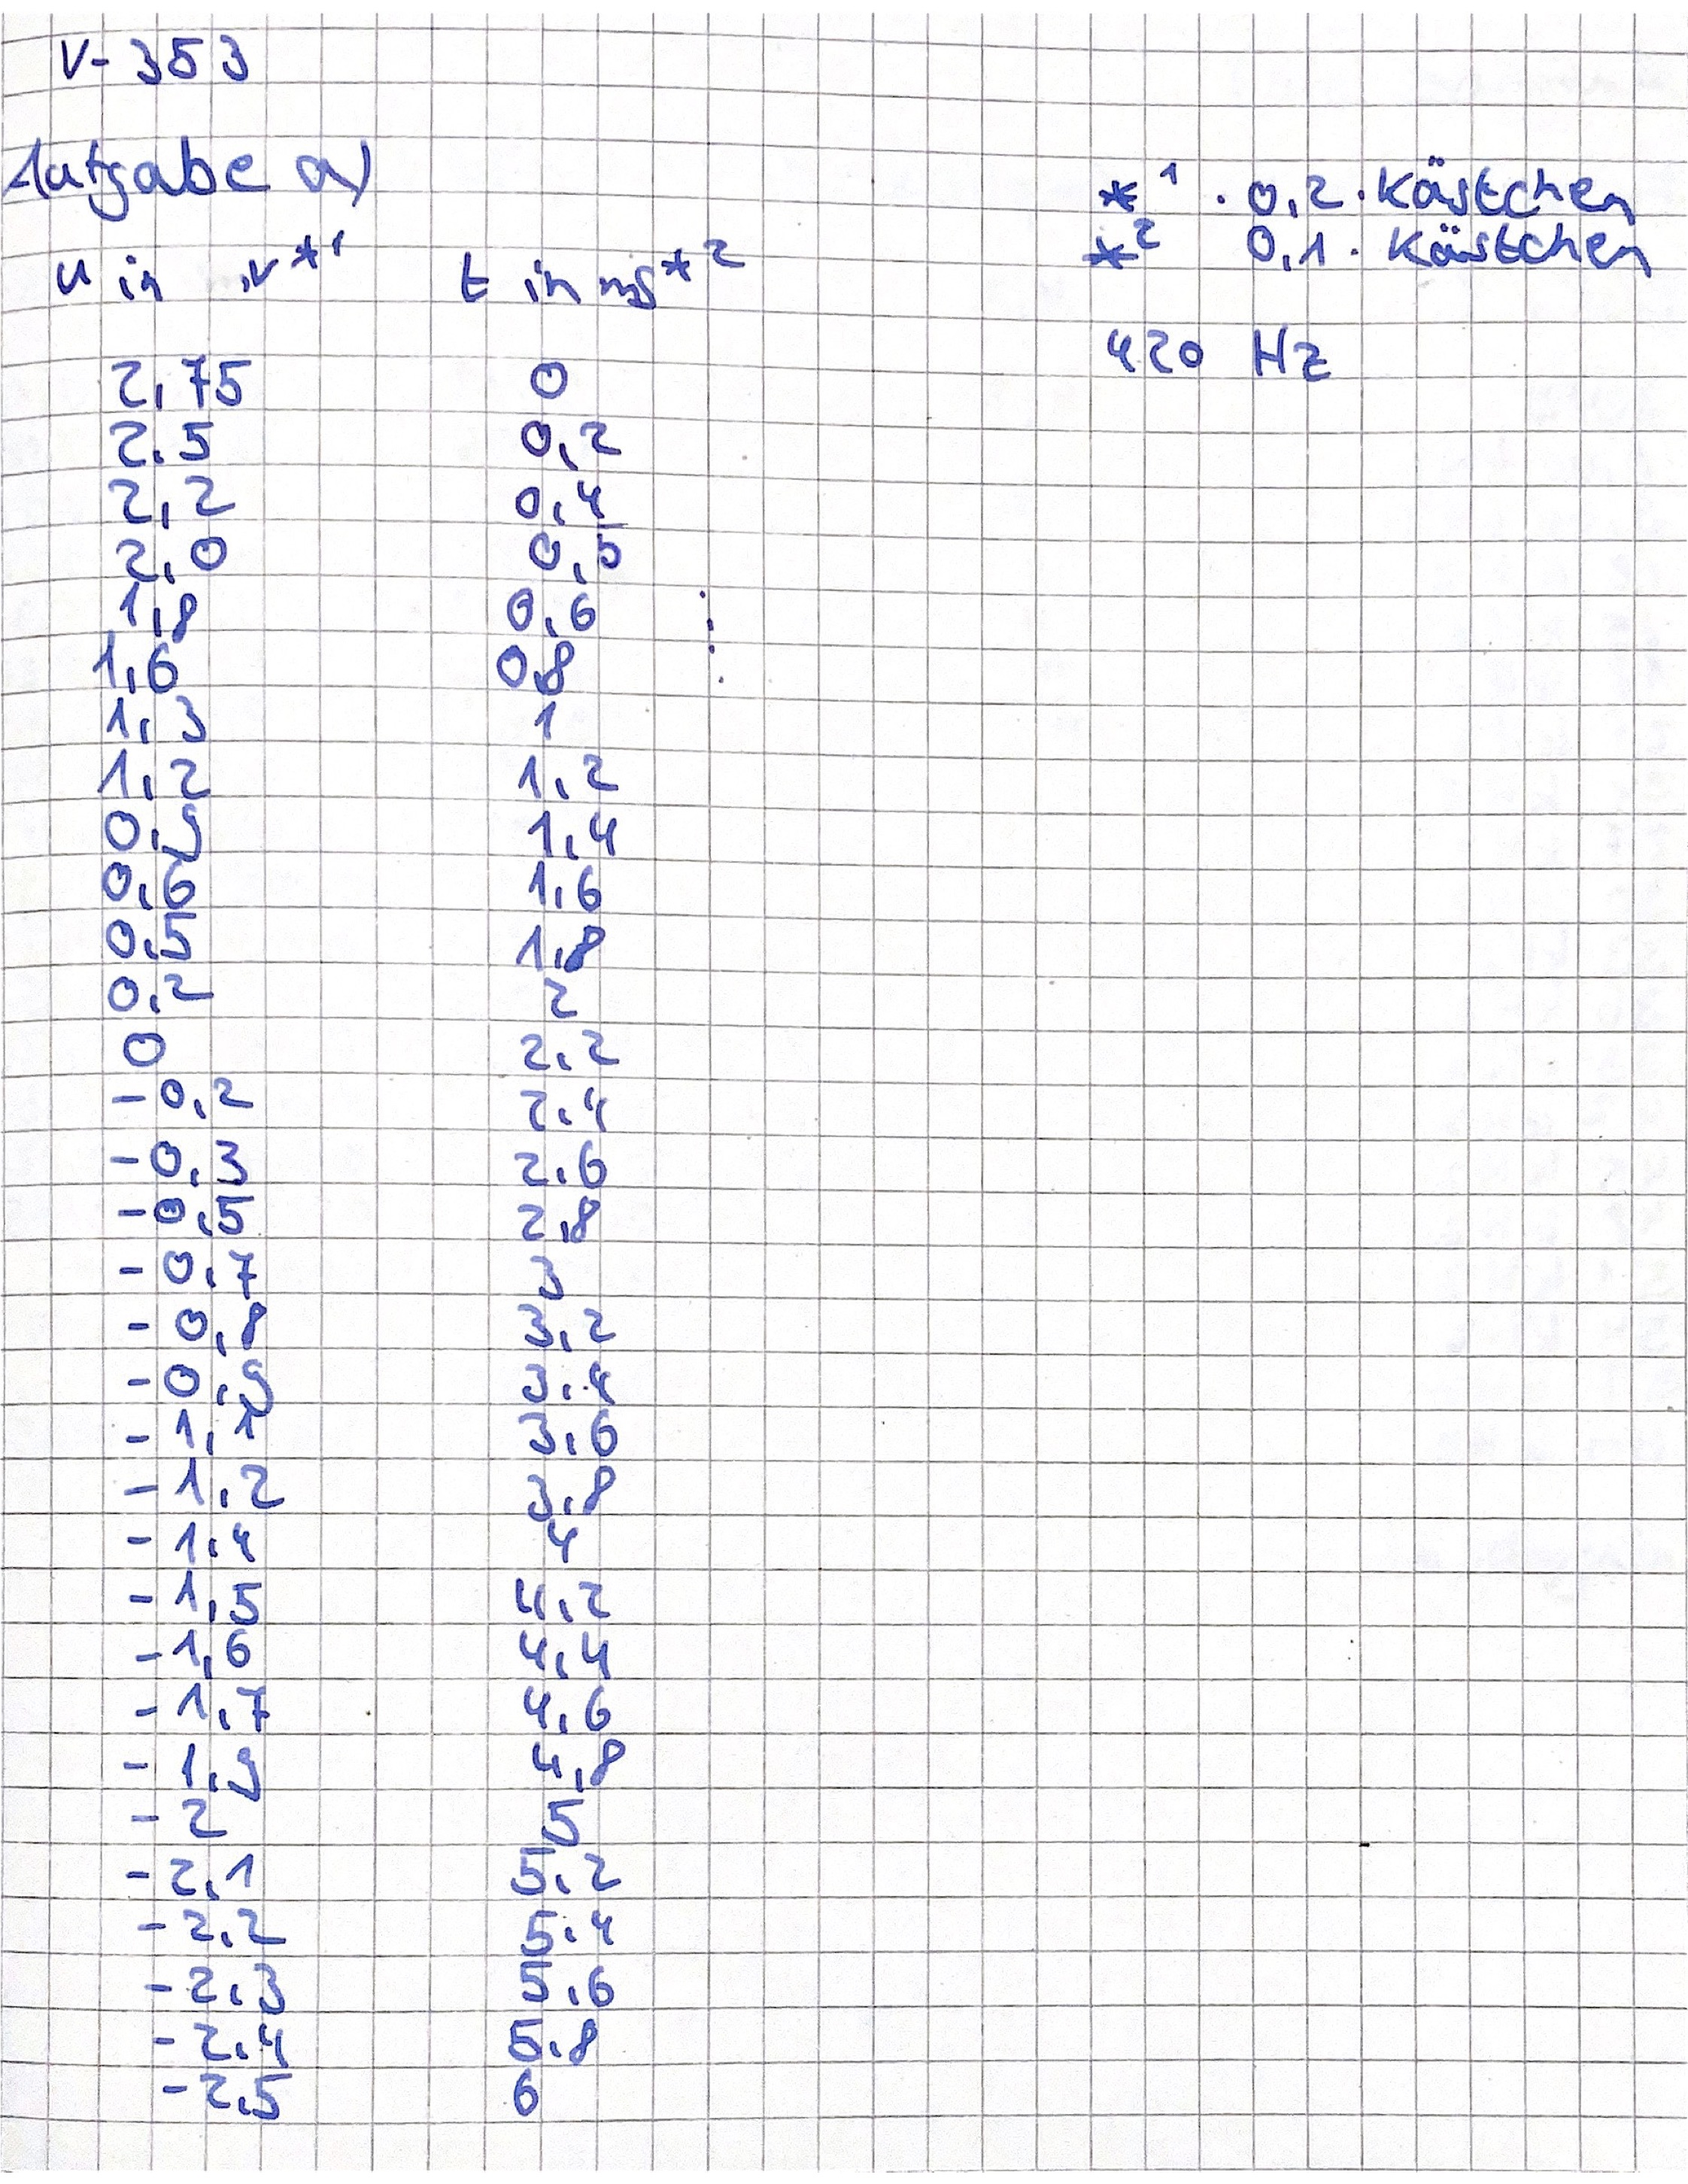
\includegraphics[width=0.75\textwidth]{Dateien/daten1.jpg}
    \caption{Originale Messdaten zu Aufgabenteil a).}
    \label{fig:daten1}
\end{figure}

\begin{figure}[H]
    \centering
    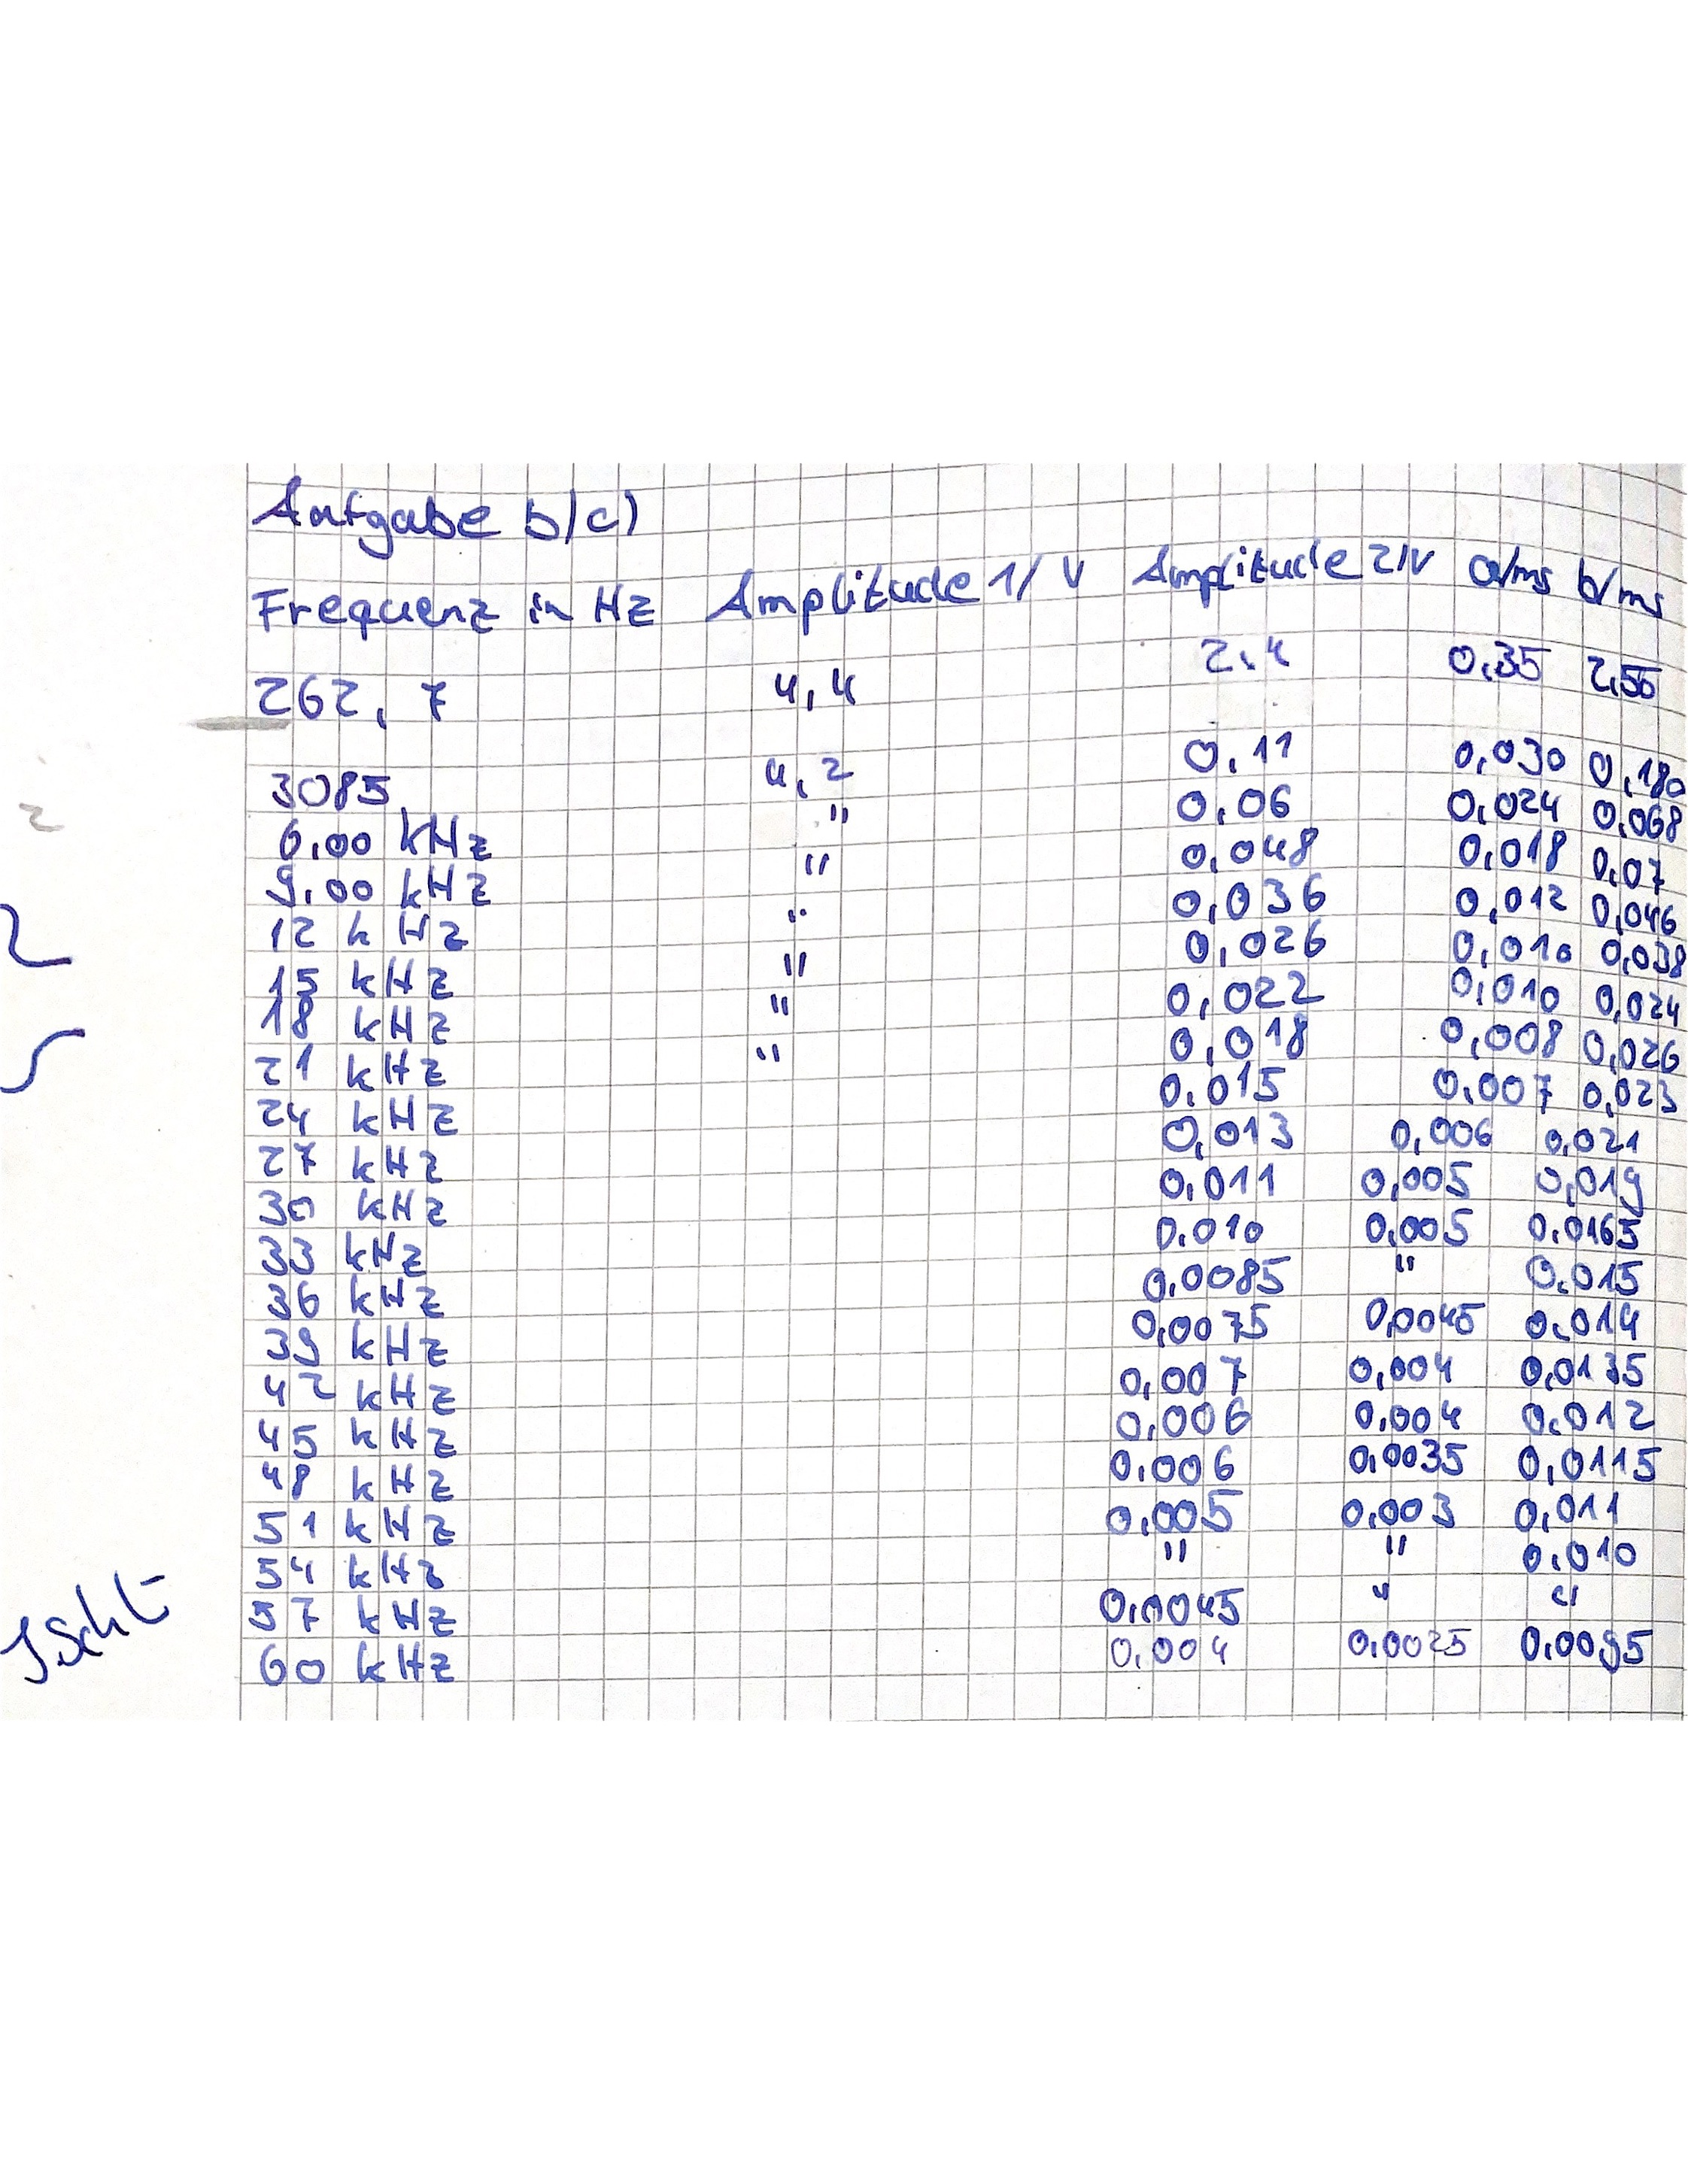
\includegraphics[width=0.75\textwidth]{Dateien/daten2.jpg}
    \caption{Originale Messdaten zu Aufgabenteil b) und c).}
    \label{fig:daten2}
\end{figure}